\documentclass[a4paper,11pt]{article}
\usepackage{polski}
\usepackage[utf8]{inputenc}
\usepackage{enumerate}
\usepackage{mathtools}
\usepackage{amsmath}
\usepackage{graphicx} 
\author{Filip Chodorowski}
\title{Sprawozdanie z laboratorium nr 4\\
„Złożoność obliczeniowa algorytmów sortowania”}
\frenchspacing
\begin{document}
\maketitle
\tableofcontents
\section{Założenia zadania}
Zadanie polegało na zaimplementowaniu wybranych algorytmów sortowania i zbadaniu ich czasu działania w zależności od ilości elementów, następnie należało je porównać.
\newpage
\section{Zaimplementowane algorytmy}
\subsection{Sortowanie przez scalanie}
Rekurencyjnie dzieli tablice na pojedyncze elementy, a następnie scala je. Podczas scalania porównuje ze sobą kolejne elementy i umieszcza w strukturze danych. Algorytm ten wymaga dodatkowego nakładu pamięci, ponieważ wykorzystywana jest struktura pomocnicza, w moim przypadku o rozmiarze danych wejściowych. Klasa złożoności obliczeniowej:
$n\log_2 n 
$
\subsection{Sortowanie Szybkie}
Kolejny algorytm rekurencyjny. Polega na wybraniu jednego elementu w tablicy, którego nazywamy osią (z ang. pivot) lub po prostu piwotem. Punkt ten można wybrać na kilka różnych sposobów. W sprawozdaniu wykorzystałem wybranie pivota skrajnie lewego lub za pomocą mediany trzech elementów: skrajnie lewego, środkowego i skrajnie prawego.
Klasa złożoności zależy tutaj od wartości danych oraz wyboru piwota i może wahać się od
$n\log_2 n 
$
do
$n^{2}
$.W przypadku pesymistycznym należy pamiętać także o fakcie, że ilość wywołań rekurencyjnych może przepełnić stos. Przypadek pesymistyczny może zajść np. podczas wyboru piwota jako skrajny element tablicy, przy danych już posortowanych. Przypadek optymistyczny ma miejsce, kiedy udaje nam się wybrać medianę z sortowanego fragmentu tablicy. W pozostałych przypadkach otrzymujemy przypadek przeciętny, który jest niewiele gorszy od przypadku optymistycznego.
\newpage
\section{Wyniki}
\subsection{Porównanie QuickSorta na Liście i Tablicy}
\begin{center}
\begin{figure}[h!]
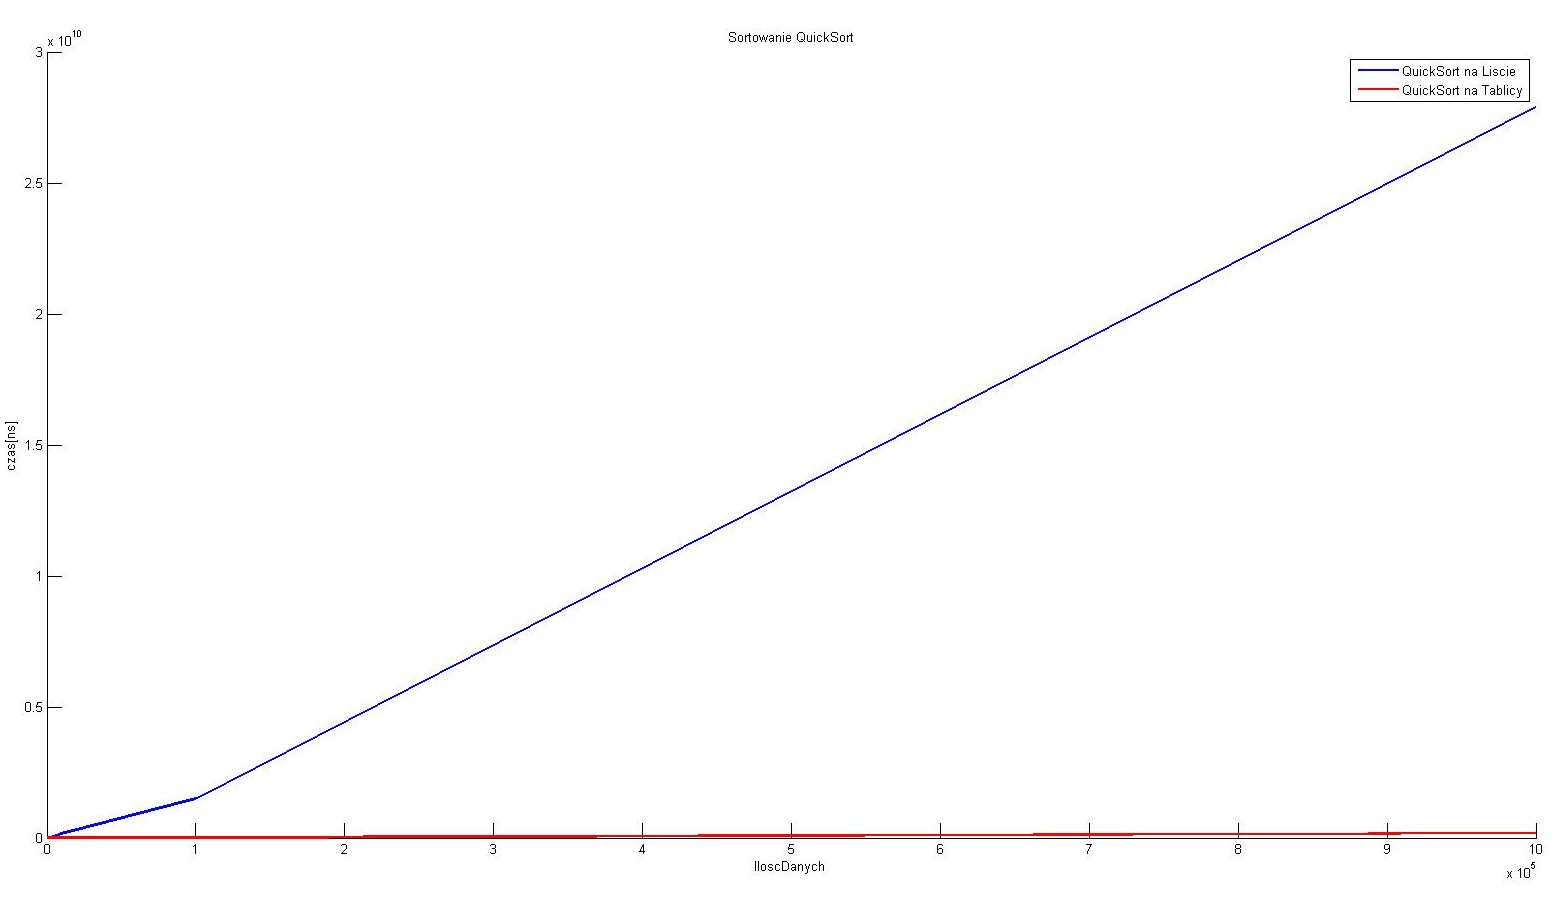
\includegraphics[width=12.5cm,height=10cm]{Wykresy2/QuickSortLista_Tablica}
%\caption{Tu umieszczasz opis}
\label{fig:obrazek Wykresy2/QuickSortLista_Tablica}
\end{figure}
\end{center}
Jak można zauważyć na wykresie czas wykonywania QuickSorta na tablicy jest zdecydowanie krótszy niż na liście, jest to różnica rzędu $10^{3}$ dla \\100 000 danych. Ta rozbieżność czasów wynika z indeksowania listy i tablicy. W quicksorcie na liście zaimplementowałem zapamiętywanie indeksów przy wywoływaniu rekurencyjnym, lecz nadal różnica jest ogromna.
\newpage
\subsection{Porównanie QuickSorta dla pivota skrajnego i wybieranego na podstawie mediany 3 elementów}
\begin{center}
\begin{figure}[h!]
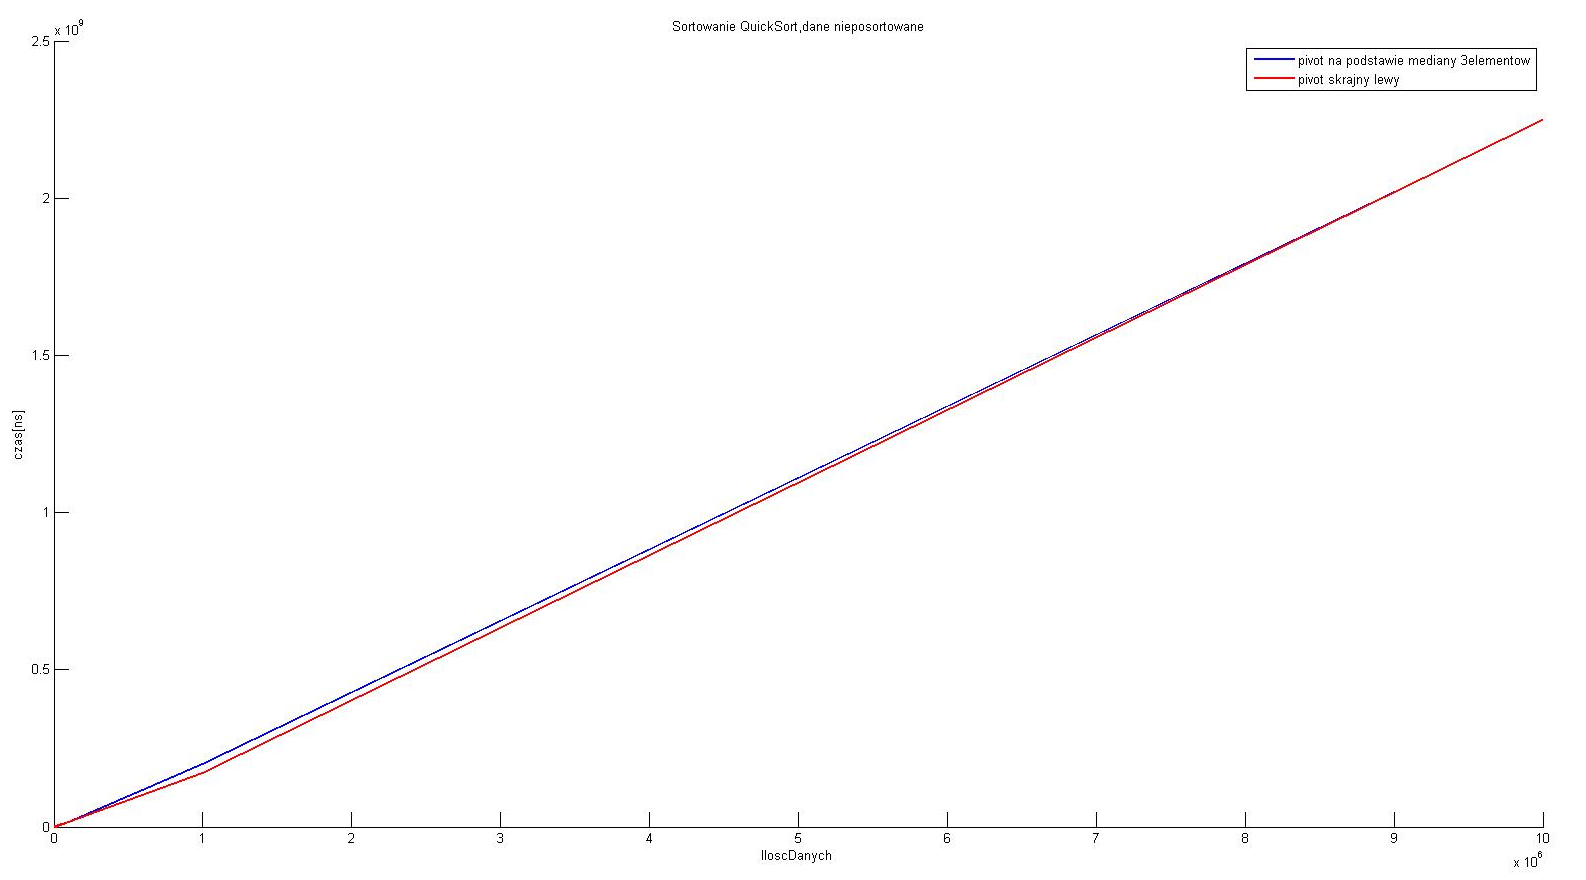
\includegraphics[width=12.5cm,height=10cm]{Wykresy2/QuickPivotyNieposortowany}
%\caption{Tu umieszczasz opis}
\label{fig:obrazek Wykresy2/QuickPivotyNieposortowany}
\end{figure}
\end{center}
Dla danych nieposortowanych, Quicksort wybierający pivot skrajny bądź też medianę na podstawie 3 elementów nie odgrywa znaczącej roli w czasie działania sortowania dla mojego algorytmu.
\newpage
\subsection{Porównanie QuickSorta dla danych posortowanych i nieposortowanych przy pivocie ustalonym jako skrajny}
\begin{center}
\begin{figure}[h!]
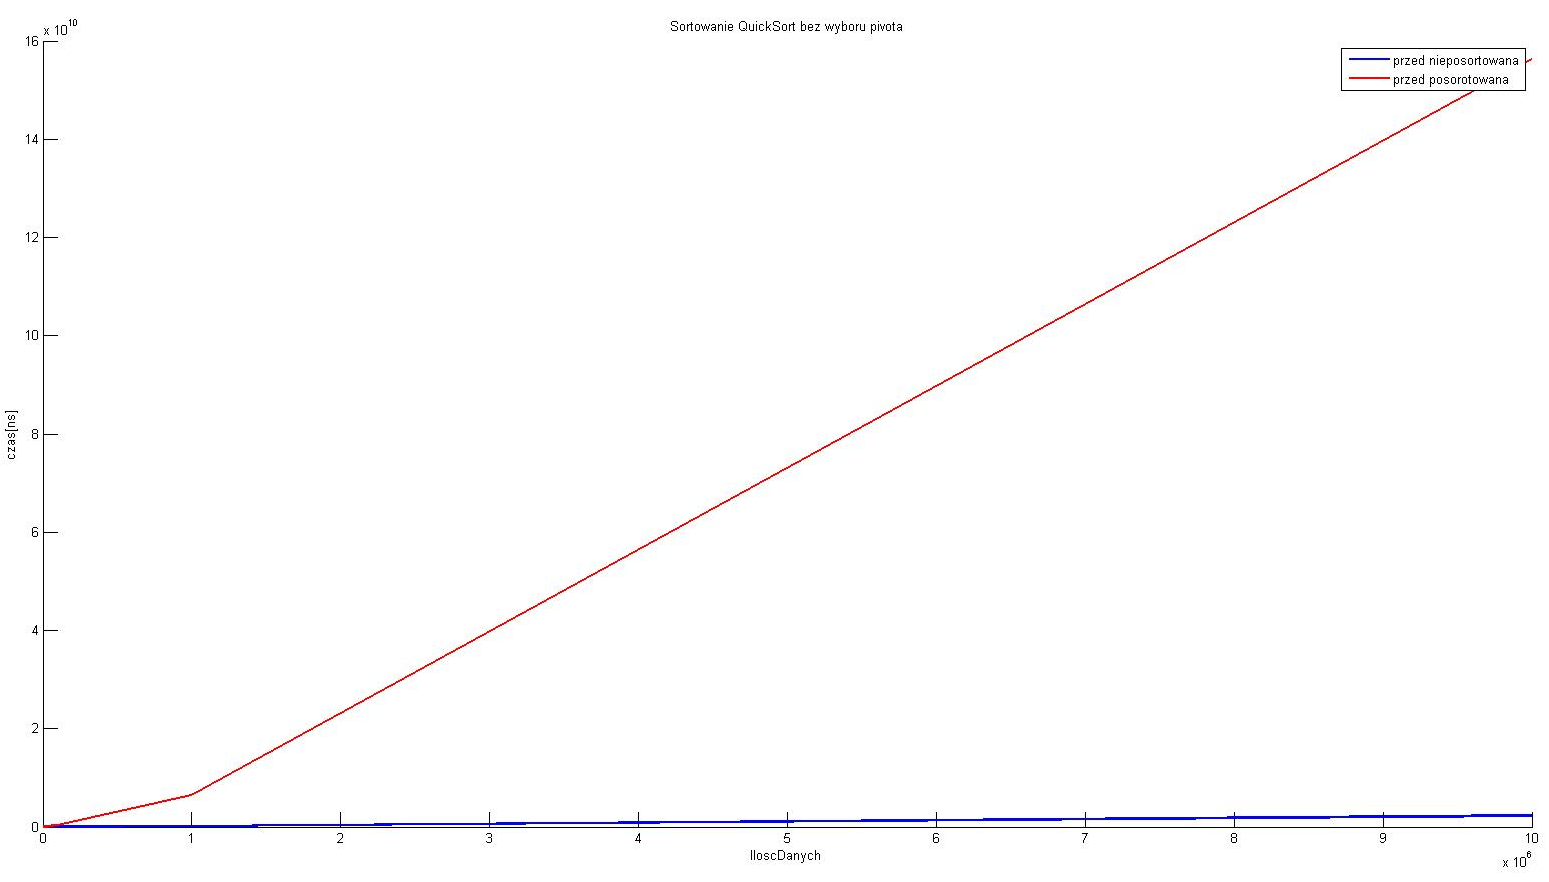
\includegraphics[width=12.5cm,height=10cm]{Wykresy2/QuickPosortowana_NieposBezPivota}
%\caption{Tu umieszczasz opis}
\end{figure}
\end{center}
Na tym wykresie można zauważyć czas działania QuickSorta dla przypadku pesymistycznego(linia czerwona), następuję on gdy zostaje wybrany skrajny piwot przy posortowanych uprzednio elementach. Różnica czasowa pomiędzy obydwoma pomiarami jest ogromna. Wynika to z faktu działania algortymu QuickSort czyli znajdowania elementu większego/mniejszego od pivota co przy posortowanej tablicy prowadzi do złożoności O($n^{2}$). 
\newpage
\subsection{Porównanie MergeSorta z QuickSortem dla danych nieposortowanych}
\begin{center}
\begin{figure}[h!]
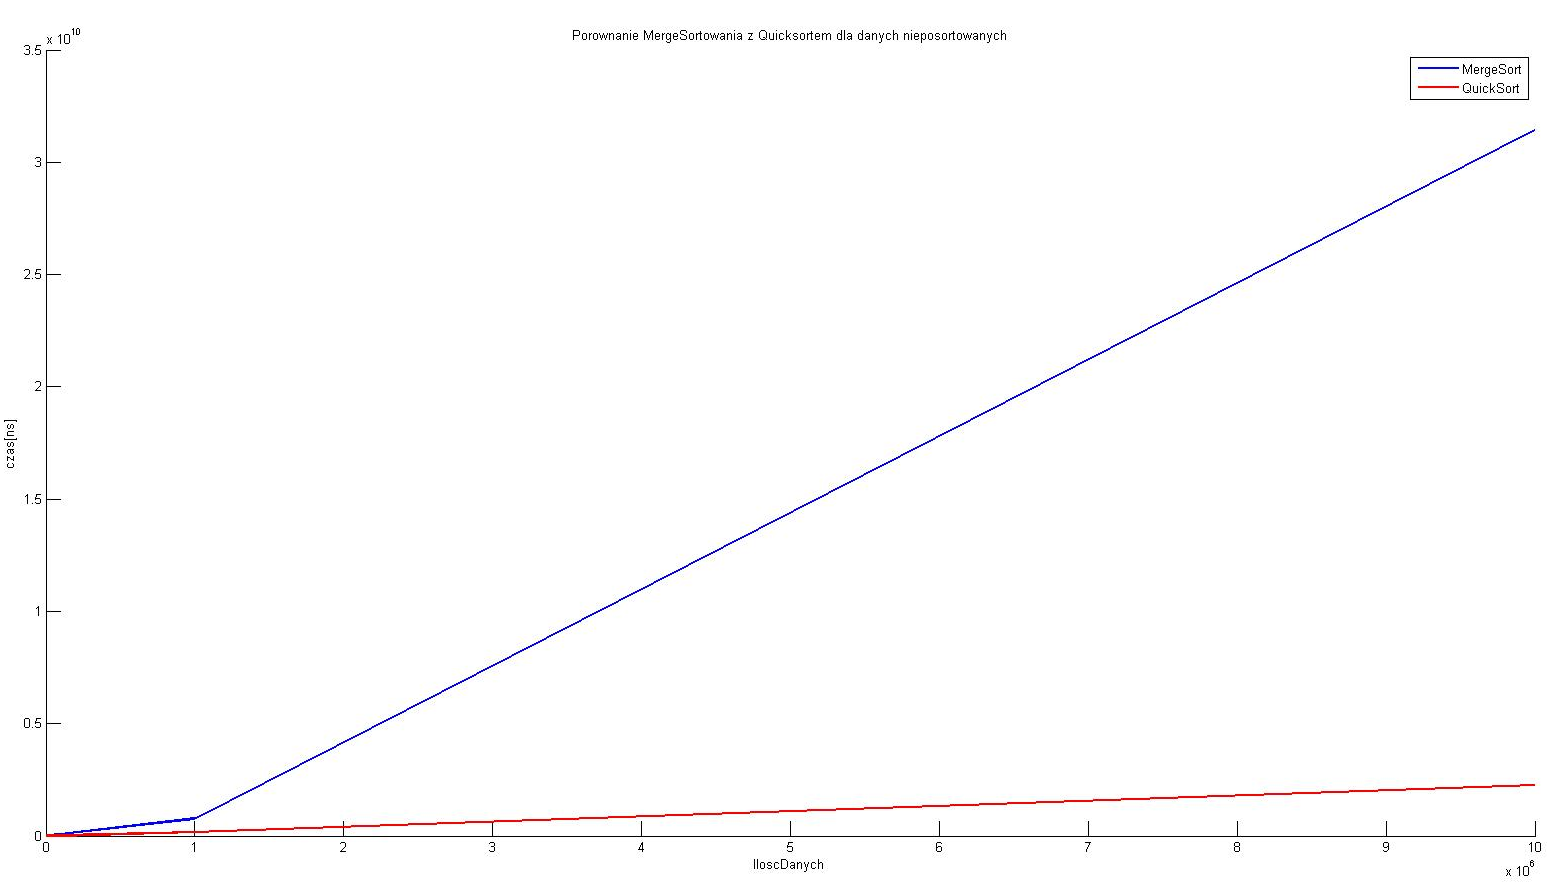
\includegraphics[width=12.5cm,height=10cm]{Wykresy2/MergeQuickNieposortowane}
%\caption{Tu umieszczasz opis}
\end{figure}
\end{center}
Dla danych nieposortowanych, Quicksort wykonuje się szybciej niż MergeSort. Algortym QuickSort  dla $10^{7}$ ilości danych wykonuje się jedynie 10 razy szybciej.
\newpage
\subsection{Porównanie MergeSorta z QuickSortem dla danych posortowanych}
\begin{center}
\begin{figure}[h!]
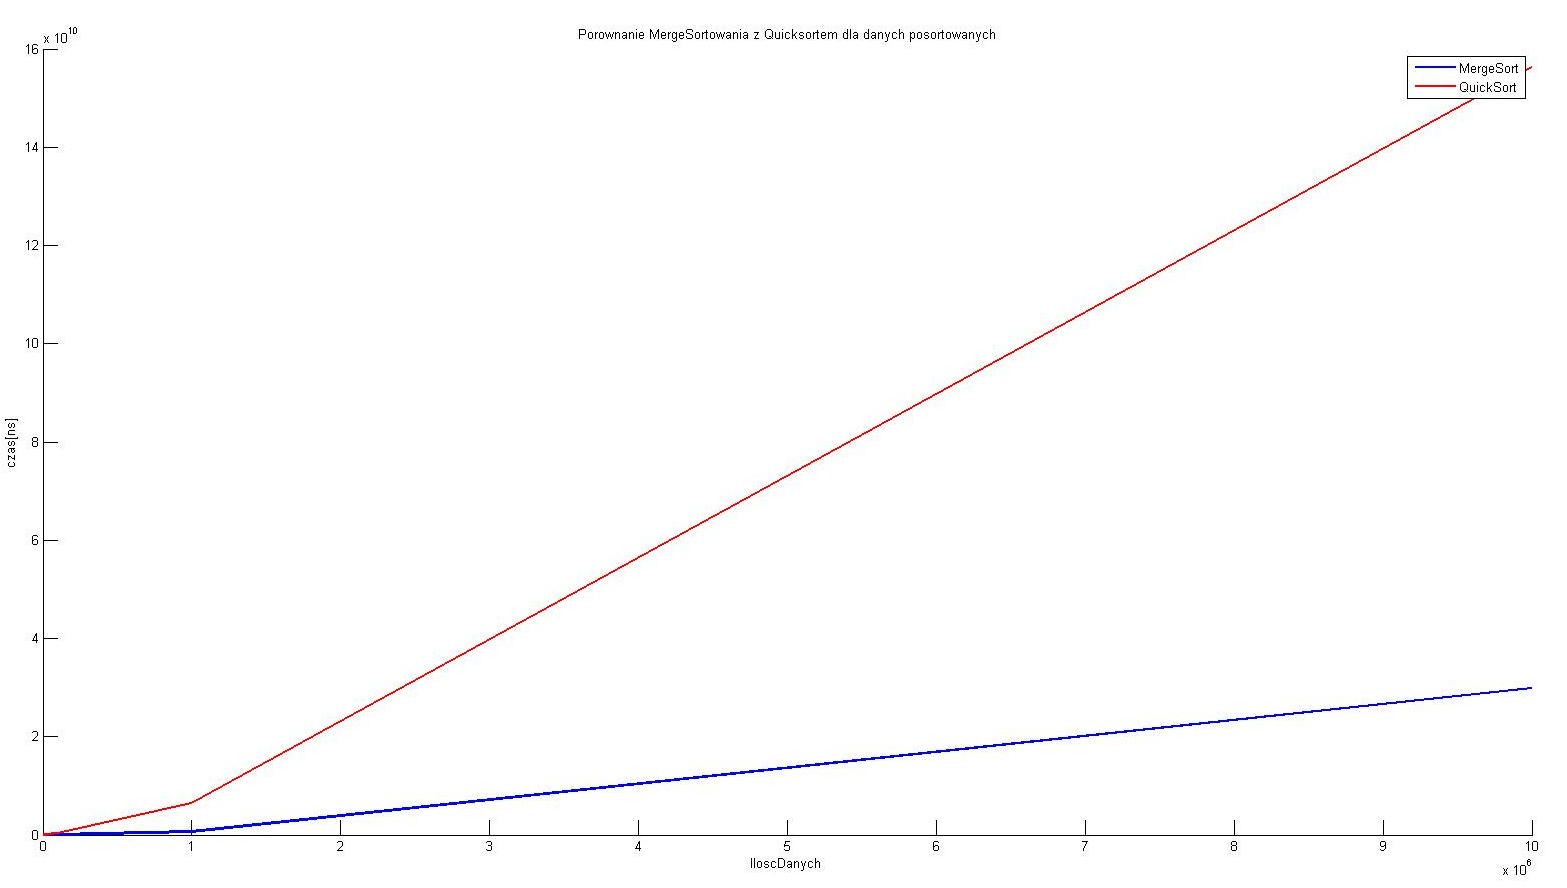
\includegraphics[width=12.5cm,height=10cm]{Wykresy2/MergeQuickPosortowane}
%\caption{Tu umieszczasz opis}
\end{figure}
\end{center}
Jak można zauważyć dla danych posortowanych, algorytm sortowania przez scalanie jest znacznie lepszy niż QuickSort(pivot skrajny).
\newpage
\subsection{Porównanie MergeSorta dla danych posortowanych i nieposortowanych}
\begin{center}
\begin{figure}[h!]
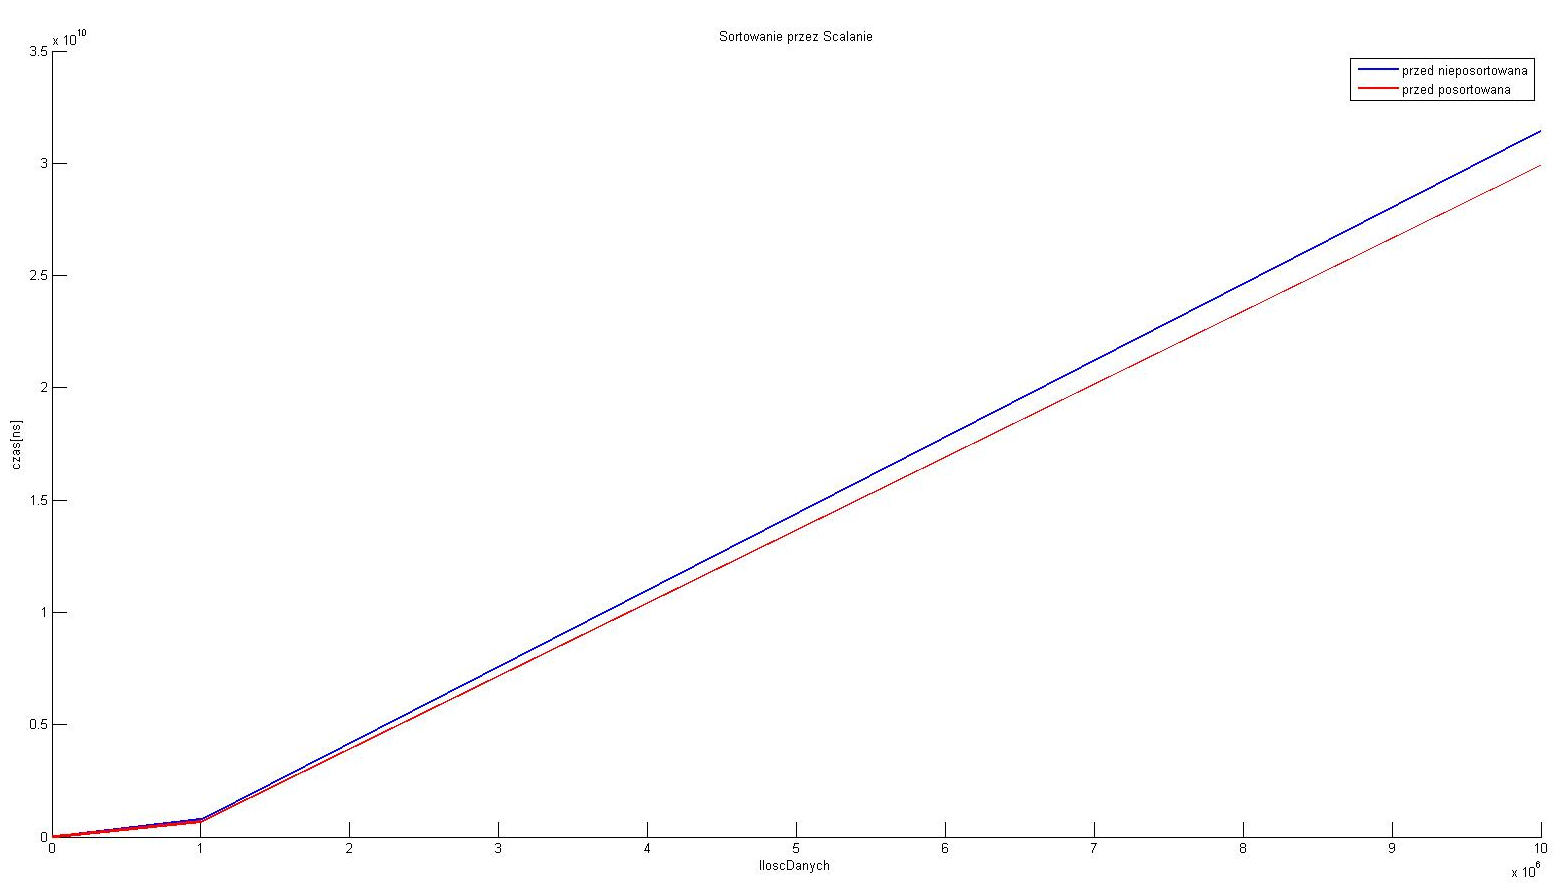
\includegraphics[width=12.5cm,height=10cm]{Wykresy2/MergeSortPosortowanaNieposortowana}
%\caption{Tu umieszczasz opis}
\end{figure}
\end{center}
Można zaobserwować zmianę w czasie działania sortowania w zależności od tego czy dane były uprzednio posortowane. Okazuję się, że trochę szybciej algorytm sortowania przez scalanie działa dla danych nieposortowanych, lecz nie następuję zmiana złożoności jak ma to miejsce w QuickSorcie.
\newpage
\section{Wnioski}
\begin{itemize}
%\ldots
\item QuickSort nie nadaje się dla struktury Lista
\item MergeSort potrzebuje dodatkowej pamięci na dane
\item Jeżeli QuickSort jest niezabezpieczony przed pesymistycznym przypadkiem, jego złożoność może gwałtownie wzrosnąć i osiągnąć O(n2)
\item W normalnym przypadku QuickSort$>$ MergeSort
\item Dla danych poniżej 50 elementów lepiej zastosować prostsze algorytmy: sortowanie przez wstawianie, bąbelkowe, bo ich złożoność jest wtedy liniowa
\end{itemize}
\end{document}